\documentclass[11pt]{article}
\usepackage[margin=1.0in]{geometry}
\usepackage{graphics,graphicx,float,subfigure,xcolor}
\usepackage{amsmath}

\DeclareMathOperator{\Tr}{Tr}
\DeclareMathOperator{\sym}{sym}
\DeclareMathOperator{\lhs}{lhs}
\DeclareMathOperator{\rhs}{rhs}
\newcommand{\RNum}[1]{\uppercase\expandafter{\romannumeral #1\relax}}
\newcommand{\red}{\textcolor{red}}
\newcommand{\blue}{\textcolor{blue}}
\newcommand{\olive}{\textcolor{olive}}

\author{
  Tozoni, Davi Colli\\
  \texttt{davi.tozoni@nyu.edu}
}
\title{Shape optimization: software and equations}

\begin{document}
\maketitle

\section{Software}

\subsection{Pipeline}

\begin{enumerate}
  \item Read \texttt{.wire} file and populate graph structures
  \item At each optimization step:
    \begin{enumerate}
      \item Inflate mesh with current truss parameters
      \item Compute the shape velocity of the boundary vertices ( in \texttt{PostProcess} + \texttt{Inflators})
      \item Solve PDE of general linear elasticity problem, finding displacement (done in similar class to \texttt{in PatternOptimizationIterate})
      \item Evaluate objective function (in similar class to \texttt{WCSObjectiveTerm})
):
        \begin{itemize}
          \item Compute function $s(\epsilon)$ corresponding to stress (e.g. $\sigma:\sigma$)           \item Compute cost function for each point $x$: $j(s) = s^{p/2}$
          \item Integrate $j(s)$ through entire function to obtain $J = \int_\Omega\, j(s(\epsilon))\, d\Omega$
        \end{itemize}
      \item Evaluate shape derivative (in class similar to \texttt{WorstCaseStress}):
        \begin{itemize}
          \item Solve adjoint cell PDE problem to find $\rho$ (used to compute $dJ[v]$)
          \item Build discrete volume differential form $dJ[v]$ 
        \end{itemize}
      \item Extend boundary shape velocities into intern nodes, in order to use $dJ[v]$ (done in \texttt{ObjectiveTerm})
      \item Compute gradient of $J$ w.r.t. shape parameters
    \end{enumerate}
    \item Output best solution found
\end{enumerate}


\subsection{Tasks based on WCS Optimization analysis}
\begin{enumerate}
  \item Create class \texttt{NonPeriodicCellOps} similar to baseCellOps to solve non periodic general PDEs
  \item Create \texttt{MicroscopicStress} class, similar to \texttt{WorstCaseStress} for computing $dJ$ and other auxiliar functions (to compute stress in our new scenario)
  \item Create \texttt{MicroscopicStressObjectiveTerm}, in a similar way to \texttt{WCSObjectiveTerm}
  \item Modify \texttt{PatternOptimizationIterate} or create similar class where general PDE is solved at each iteration, (by calling \texttt{NonPeriodicCellOps})
\end{enumerate}

The interaction works as following: class \texttt{MicroscopicStressObjectiveTerm} uses \linebreak\texttt{NonPeriodicCellOps} of \texttt{PatternOptimizationIterate} (after solving PDE) to evaluate objective term and compute differential. The iterate class (4) then should be used by the \texttt{IterateManager} class inside the solvers.



\section{Our problem}
In this project, the objective is to solve a general shape optimization problem, given fixed Dirichlet and Neumann boundary conditions, as represented in the picture below:

  \begin{figure}[hbt]
    \begin{center}
      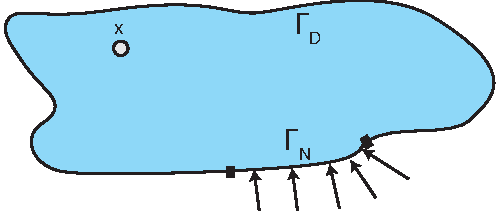
\includegraphics[width=0.75\textwidth]{figures/problem}
    \end{center}
    \caption{Our problem.}
    \label{fig:problem}
  \end{figure}

The corresponding PDE then is the following (strong form):
\begin{align*}
  - \nabla & \cdot \sigma = 0 \text{ (external force)} \\
  &\text{such that: } \\
  &u =  \hat u \quad \text{ on $\Gamma_D$}\\
  &\sigma n = \hat T \quad \text{ on $\Gamma_N$}
\end{align*}
, where $u$ is the unknown displacement, $\epsilon = 1/2 (\nabla u + (\nabla u)^T)$ is the strain and $\sigma = C \epsilon$ is the stress.

The corresponding weak form is the following:
\begin{equation}
\int_\Omega\, \epsilon(\phi) : C : \epsilon(u)\, dw = \int_{\Gamma_N} \phi \cdot \hat T\, d\Gamma_N
  \label{eq:weakform}
\end{equation}
, for all $\phi$ where $\phi(y) = 0 \quad \forall \:  y \in \Gamma_D$. \blue{The corresponding weak form for the periodic case can be found in equation (A1) in \cite{panetta2017}}.

Now, consider we are minimizing a cost function $\int_\Omega\, j(s(u))\, dx$, where $s$ corresponds to some measure of stress, and $j(s) = s^{p/2}$. In summary, we are optimizing the $L^p$ norm of the stress in the whole object.

In the remaining of this text, I suppose $s(u) = \| \sigma \|^2_F = \sigma^T : \sigma = \sigma : \sigma$. Notice that operation $A:B$ equals $A_{ij} B_{ij}$ in index notation (for $A$ and $B$ being 2-order tensors).

The computation of the cost itself is not difficult and can be done directly through a quadrature rule after solving our original elasticity PDE. However, when optimizing the shape, we need to compute how cost changes when deforming the $\Omega$. This means computing the \textbf{\emph{shape derivative}} of $J$.

So here are the steps:
\begin{enumerate}
  \item Find equation of $dJ[v]$
  \item Compute $\tau$, which corresponds to the derivative of $j$ with respect to strain $\epsilon$
  \item Compute derivative of our PDE weak form
  \item Find adjoint PDE for computing continuous version of $dJ[v]$
  \item Compute discrete differential form for $dJ[v]$ (the one that is actually implemented)
\end{enumerate}

\subsection{Find Equation for $dJ[v]$}
Consider the mapping $f_t(X) = X + t v(X)$ represented in the Figure \ref{fig:mapping}, where $v$ is the velocity. (The inverse of $f_t$ is then $f_t^{-1}(x) = x - tv$). 

The jacobian of the map is then $\nabla f_t$ and equals $F_t = I + t\nabla v$. (As we know, the jacobian of $f_t^{-1}$ corresponds to $F_t^{-1}$).

  \begin{figure}[hbt]
    \begin{center}
      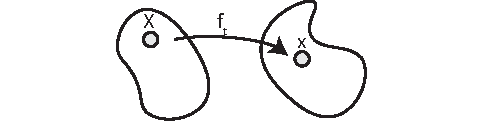
\includegraphics[width=0.8\textwidth]{figures/mapping}
    \end{center}
    \caption{Mapping between initial and deformed object after time $t$.}
    \label{fig:mapping}
  \end{figure}

We can compute the displacement $u$ of a point $x$ (after time $t$) as $u_t(x)$, which equals function $\hat u(X)$ with domain $\Omega_0$: 
$$
  u_t(x) = \hat u(X) = \hat u(x - tv)
$$
As a consequence, we also have that:
$$
  \epsilon(u_t(x)) = \epsilon(\hat u (x - tv)) = \epsilon(\hat u (f_t^{-1}(x))) = \epsilon(\hat u(X))
$$

Applying this to our cost $J$, we can obtain a formula entirely on $\Omega_0$, facilitating derivatives w.r.t. time:
$$
J = \int_{\Omega(t)} j(s(\epsilon(u_t(x)))) dx = \int_{\Omega_0} j(s(\epsilon(\hat u (X) ) ) ) \det(\nabla f_t) dX
$$

Deriving $J$ w.r.t $t$:
\begin{align*}
  \frac{dJ}{dt} &= \int_{\Omega_0} \frac{d}{dt} \left( j(s(\epsilon(\hat u (X) ) ) ) \det(\nabla f_t) \right) dX\\
  &= \int_{\Omega_0} \tau : D[\epsilon] \det(F_t) + j \det(F_t) \Tr(F_t^{-1} \nabla v) dX
\end{align*}
, where $D[\cdot]$ is the material derivative of $\cdot$ and $\tau = \frac{\partial j}{\partial s} \frac{\partial s}{\partial \epsilon}$.

We can then compute the shape derivative by evaluating the derivative at $t=0$. Notice that $F_0 = I$ and that $\Tr(\nabla v) = \nabla \cdot v$.
\begin{align*}
  dJ[v] = \frac{dJ}{dt} \Big|_{t=0} &= \int_{\Omega_0} \tau : D[\epsilon] + j \nabla \cdot v \, dX
\end{align*}

But $D[\epsilon(u)]$ can be written as $\epsilon(D[u]) - \sym(\nabla u \nabla v)$, where $\sym[\cdot]$ means the symmetric part of $\cdot$. Plugging this, we obtain the equation below:
\begin{equation}
  \boxed{dJ[v] = \int_{\Omega_0} \underbrace{\tau : \epsilon(D[u])}_{\RNum{3}} - \tau : \sym(\nabla u \nabla v) + j \nabla \cdot v \, dX}
  \label{eq:dJ}
\end{equation}
, \blue{which corresponds to formula (A17) in the supplementary material of \cite{panetta2017}.}

As expected, term $\RNum{3}$ is the difficult one to compute, since $u$ is the output of a PDE.

\subsection{Compute $\tau$}

Let's compute $\tau$:
\begin{align*}
  \tau = j' \frac{\partial s}{\partial \epsilon}  
\end{align*}

It is easier to compute for each entry in $\tau$ the following way:
\begin{align*}
  \tau_{ij} &= j' \frac{\partial s}{\partial \epsilon_{ij}} = j' \frac{\partial s}{\partial \epsilon_{ij}}( \sigma : \sigma )  = j' \left( \frac{\partial \sigma}{\partial \epsilon_{ij}}: \sigma + \sigma :   \frac{\partial \sigma}{\partial \epsilon_{ij}} \right) \\
  &= 2j' \frac{\partial \sigma}{\partial \epsilon_{ij}}: \sigma = 2j' C^{\text{base}} : \frac{\partial \epsilon}{\partial \epsilon_{ij}} : \sigma
\end{align*}

But $\frac{\partial \epsilon_{kl}}{\partial \epsilon_{ij}} = \delta_{ki}\delta_{lj}$ and then:

$$
  \frac{\partial (C_{abcd}\epsilon_{cd})}{\partial \epsilon_{ij}} = C_{abij}
$$

Consequently, $\tau_{ij} = 2j' (\sigma_{ab} C_{abij})$ and
\begin{equation}
  \boxed{\tau = 2j' \sigma : C}
  \label{eq:tau}
\end{equation}
, \blue{which corresponds to equation (A10) in \cite{panetta2017}.}

\subsection{Compute Derivative of PDE}

In order to compute term $\RNum{3}$, we need to compute the derivative of the weak form in Equation \ref{eq:weakform}, as shown here.

We start with the weak form:
$$
\int_\Omega\, \epsilon(\phi) : C : \epsilon(u)\, dX = \int_{\Gamma_N} \phi \cdot \hat T\, d\Gamma_N
$$

Differentiating on both sides (and obtaining the value at $t=0$):
\begin{align*}
  \underbrace{\frac{d}{dt} \Big|_{t=0} \left( \int_\Omega\, \epsilon(\phi) : C : \epsilon(u)\, dX \right)}_{\text{lhs}} = \underbrace{\frac{d}{dt} \Big|_{t=0} \left( \int_{\Gamma_N} \phi \cdot \hat T\, d\Gamma_N\right)}_{\text{rhs}}
\end{align*}

\subsubsection{Computing left hand side:}
Similar math to derivation of $dJ$:
\begin{align*}
  u(x) = \hat u(x - tv) \text{ and } \phi(x) = \hat \phi(x - tv)  
\end{align*}
  
\begin{align*}
  \lhs = \int_{\Omega_0} \frac{d}{dt}\Big|_{t=0}  \left( \epsilon(\hat \phi):C:\epsilon(\hat u) \right) \det(F_0) + \epsilon(\hat \phi):C:\epsilon(\hat u) \frac{d}{dt} \Big|_{t=0} \left(\det(F_t)\right) dX
\end{align*}

Applying product rule on first term and using that $\frac{dA_t}{dt} = det(A_t)\Tr(A_t^{-1} \frac{\partial A_t}{\partial t})$ , we obtain:
\begin{align*}
  \lhs = \int_{\Omega_0} \left( D[\epsilon(\hat \phi)]:C:\epsilon(\hat u) + \epsilon(\hat \phi):C:D[\epsilon(\hat u)] + \epsilon(\hat \phi): C : \epsilon(\hat u) \nabla \cdot v \right) dX
\end{align*}

Because $D[\epsilon(w)] = \epsilon(D[w])  - \sym(\nabla w \nabla v)$, we have:
\begin{align*}
  \lhs &=  \int_{\Omega_0} \left((\epsilon(D[\phi])  - \sym(\nabla \hat \phi \nabla v)):\underbrace{C:\epsilon(\hat u)}_{\sigma} + \epsilon(\hat \phi):C:(\epsilon(D[u])  - \sym(\nabla \hat u \nabla v)) + \epsilon(\hat \phi): \underbrace{C : \epsilon(\hat u)}_{\sigma} \nabla \cdot v \right) dX\\
  &= \int_{\Omega_0} \left((\epsilon(D[\phi])  - \sym(\nabla \hat \phi \nabla v)):\sigma + \epsilon(\hat \phi):C:(\epsilon(D[u])  - \sym(\nabla \hat u \nabla v)) + \epsilon(\hat \phi): \sigma \nabla \cdot v \right) dX
\end{align*}

In our case, since $\phi$ are functions of the barycentric coordinate functions in our FEM, $D[\phi] = 0$. In other words, $\phi(x) = \sum_i \phi_i(x)$ depends only on $x$ and not on $t$. \textcolor{red}{But $x$ depends on $t$, doesn't it? The material point $x$ doesn't! Actually, $\phi$ depends on how $x$ is positioned related to its neighbors, which does not change after time $t$, since $x$ continue being a weight average of its face vertices (with same weights always). Would any of this change if we were using a non linear basis function for the FEM?}.

Finally,
\begin{align*}
  \lhs &= \int_{\Omega_0} \left(- \sym(\nabla \hat \phi \nabla v)):\sigma + \epsilon(\hat \phi):C:(\epsilon(D[ u])  - \sym(\nabla \hat u \nabla v)) + \epsilon(\hat \phi): \sigma \nabla \cdot v \right) dX
\end{align*}

\subsubsection{Computing right hand side:}
We know:
\begin{align*}
  \hat T_t(x) = \hat T(x - tv) \text{ and } \phi(x) = \hat \phi(x - tv)  
\end{align*}

And we aim to compute the following integral
\begin{align*}
  \rhs = \frac{d}{dt} \Big|_{t=0} \left( \int_{\Gamma_N} \phi \cdot \hat T_t\, d\Gamma_N\right)
\end{align*} 

Then
\begin{align*}
  \rhs &= \int_{\Gamma_{N_0}} \frac{d}{dt} \Big|_{t=0} \left(\hat \phi \cdot \hat T \det(F_t) \right)\, d\Gamma_{N_0}\\
  &= \int_{\Gamma_{N_0}} ( \underbrace{D[\phi]}_{\textbf{0} \text{ (FEM)}} \cdot \hat T + \phi \cdot \underbrace{D[\hat T]}_{\textbf{0} \text{ (b.c.)}} ) \det(F_0) + \hat \phi \cdot \hat T \frac{d}{dt} \Big|_{t=0}\left(\det(F_t)\right) d\Gamma \\
  &= \int_{\Gamma_{N_0}} \hat \phi \cdot \hat T \quad \nabla \cdot v\, d\Gamma_{N_0}
\end{align*}

\subsubsection{Combining results}
At $t=0$, $\hat u = u$ and $\hat \phi = \phi$. Then, combining the left and right hand sides:
\begin{align*}
  \int_{\Omega_0} \left(- \sym(\nabla \phi \nabla v)):\sigma + \epsilon(\phi):C:(\epsilon(D[u])  - \sym(\nabla u \nabla v)) + \epsilon(\phi): \sigma \nabla \cdot v \right) dX = \int_{\Gamma_{N_0}} \phi \cdot \hat T \quad \nabla \cdot v\, d\Gamma_{N_0}
\end{align*}

And
{\small
\begin{equation}
  \boxed{\int_{\Omega} \epsilon(\phi):C:\epsilon(D[u]) dX =
  \int_{\Omega} \sym(\nabla \phi \nabla v):\sigma + \epsilon(\phi):C:\sym(\nabla u \nabla v) - \epsilon(\phi): \sigma \nabla \cdot v  dX + \int_{\Gamma_{N}} \phi \cdot \hat T \quad \nabla \cdot v\, d\Gamma_{N}}
  \label{eq:forwardversion}
\end{equation}
}
You can think this equation a weak form of another PDE on $D[u]$. However, we would have to solve a different PDE for each $v$. \blue{This corresponds to formula A(19) in \cite{panetta2017}}.

\subsection{Adjoint PDE Problem}
We can then try to find the value of equation $\RNum{3}$ in another way, with an adjoint version of the original PDE.

Initially, consider we have the following PDE with unknown $\rho$:
\begin{equation}
  \int_\Omega \tau:\epsilon(\psi)\, dx = \int_\Omega \epsilon(\rho):C:\epsilon(\psi) \, dx 
  \label{eq:adjointproblem}
\end{equation}
, where $\rho$ is from the same function space as $\phi$ (meaning it equals $0$ on Dirichlet boundary) and $\psi$ is from the same space as $D[u]$. \textcolor{red}{Since $\psi$ is used as test function here, it should be $0$ at $\Gamma_D$, but how can we ensure it happens? Since values at Dirichlet boundary does not change, the material derivative is then $0$, agreeing with what should happen to the test functions at $\Gamma_D$}.

The corresponding strong form of this weak formulation would be:
\begin{align*}
  - \nabla & \cdot \sigma(\rho) = - \nabla \cdot \tau \\
  &\text{such that: } \\
  &\rho =  0 \text{ on $\Gamma_D$}\\
  &\sigma(\rho) n = \tau n \quad \text{ on $\Gamma_N$}
\end{align*}


Then, after finding $\rho$, we could compute $\RNum{3}$ using the forward PDE Equation \ref{eq:forwardversion} and the following:
\begin{align*}
  \RNum{3} = \int_\Omega \tau:\epsilon(D[u])\, dx = \int_\Omega \epsilon(\rho):C:\epsilon(D[u]) \, dx
\end{align*}

Obtaining:
\begin{equation}
  \boxed{\RNum{3} =
  \int_{\Omega} \sym(\nabla \rho \nabla v):\sigma + \epsilon(\rho):C:\sym(\nabla u \nabla v) - \epsilon(\rho): \sigma \nabla \cdot v  dX + \int_{\Gamma_{N}} (\rho \cdot \hat T) \quad \nabla \cdot v\, d\Gamma_{N}}
  \label{eq:IIIcomputation}
\end{equation}

Combining this with Equation \ref{eq:dJ}, and noticing we can drop the $\sym$ operation (because its output is always double contracted with a symmetric tensor):
\begin{multline}
  \boxed{dJ[v] = \int_{\Omega} (j - \epsilon(\rho): \sigma)\nabla \cdot v + (\nabla \rho \nabla v):\sigma + (\epsilon(\rho):C - \tau) : (\nabla u \nabla v) \, dX } \\ \boxed{+ \int_{\Gamma_{N}} (\rho \cdot \hat T) \quad \nabla \cdot v\, d\Gamma_{N}  }
  \label{eq:completedJ}
\end{multline}

\blue{The corresponding formulas for the periodic case can be found in section 3.1.2 of the suplementarial material of \cite{panetta2017}.}

\subsection{Discrete Differential Form for $dJ_d[v]$}

The input of the differential form is a velocity vector field $v(x)$. It is discretized considering velocities $\delta q_m$ on the vertices of our input mesh $v(x) = \sum_m \lambda_m(x) \, \delta q_m$. Note that, despite being a global formula, only values of vertices close to $x$ should affect $v(x)$ (which usually means $\lambda_m(x)$ is different than $0$ only if $m$ is in the face containing $x$).

At the same time, $\rho$ and $u$ are discretized in similar manner, but using the $n$ FEM nodes created during the simulation. Summarizing, we have:
\begin{align*}
    v(x) &= \sum_m \lambda_m(x) \, \delta q_m\\
    u(x) &= \sum_n \varphi_n(x) \, u_n\\
    \rho(x) &= \sum_n \varphi_n(x) \, \rho_n
\end{align*}

We can then imply some important properties:
\begin{align*}
    \nabla v &= \sum_m   \delta q_m \otimes \nabla \lambda_m\\
    \nabla \rho &= \sum_n   \rho_n \otimes \nabla \varphi_n\\
    \nabla u &= \sum_n   u_n \otimes \nabla \varphi_n\\
    \nabla \cdot v &= \sum_m   \nabla \lambda_m \cdot \delta q_m\\    
    \nabla \rho \nabla v &= \sum_{m,n} (\rho_n \otimes \nabla \varphi_n)(\delta q_m \otimes \nabla \lambda_m)\\
    \tau:(\nabla \rho \nabla v) &= \sum_m \delta q_m \cdot (\sum_n \left[ \nabla \lambda_m \cdot (\tau \rho_n) \right] \nabla \varphi_n)\\
    (\nabla \rho \nabla v):\sigma &= \sum_m \delta q_m \cdot (\sum_n \left[ \nabla \lambda_m \cdot (\sigma \rho_n) \right] \nabla \varphi_n)
\end{align*}

Let's consider again $dJ[v]$:
\begin{align*}
  dJ[v] = \int_{\Omega} \olive{(\nabla \rho \nabla v}):\sigma + \epsilon(\rho):C:\olive{(\nabla u \nabla v)} - \epsilon(\rho): \sigma \olive{\nabla \cdot v}  - \olive{\tau : (\nabla u \nabla v)} + j \olive{\nabla \cdot v} \, dX \\ + \int_{\Gamma_{N}} \rho \cdot \hat T \quad \olive{\nabla \cdot v}\, d\Gamma_{N}
\end{align*}

Now, let's apply our transformations for discrete $v$, $u$ and $\rho$ to obtain $dJ_d$.
\begin{equation}
  \boxed{dJ_d[\lambda_m \delta q_m] = \underbrace{\left( \int_\Omega \left[ j - \epsilon(\rho):\sigma \right] \nabla \lambda_m + \left[ \nabla \lambda_m \cdot (\sigma p_n + (\epsilon(p):C-\tau)u_n) \right] \nabla \varphi_n dx + \int_{\Gamma_N} (\rho \cdot \hat T) \nabla \lambda_m d\Gamma \right)}_{dJ_m} \cdot \delta q_m}
\end{equation}
, \blue{which corresponds to final formula of Section 3.1.3 of Supplementary Material of \cite{panetta2017}}.

With this formula, all you have to do in order to compute $dJ_d$ is to sum the dot products of $dJ_m$ with the velocity $m$ ($\delta q_m$) for all mesh vertices.


\bibliographystyle{abbrv}
\bibliography{shape-optimization} 

\end{document}